\chapter{Introdução}

\section{Motivação}
Há uma expectativa de que, no ano de 2017, o número de casas inteligentes aumente cerca de 17\% nos Estados Unidos \cite{mckinseyReport}, onde já se tem investimentos de grandes empresas, como Google, Amazon e Apple. O interesse nessa área é tamanho que a Google investiu cerca de 5 milhões de dólares em um comercial de seu produto Google Home no Super Bowl 2017, jogo que decide o time campeão da temporada de futebol americano nos EUA \cite{kennemer}. É esperado que os consumidores invistam cada vez mais em casas inteligentes nos próximos anos, com previsões de que o valor total desse mercado chegue a mais de 63 bilhões de dólares em 2020 \cite{businessWire}.

As aplicações de automação residencial não mais se limitam aos sistemas de iluminação, controle da ventilação e temperatura de cômodos. Elas contemplam também segurança, eficiência energética e até mesmo soluções voltadas à área da saúde, com dispositivos desenvolvidos especificamente para pessoas idosas, com problemas de mobilidade ou doenças crônicas \cite{iscoop}.

Os avanços das tecnologias de Internet das Coisas (\textit{Internet of Things} ou \wiot{}) apontam para um futuro no qual qualquer dispositivo da casa possa estar conectado à Internet, onde surge uma série de possibilidades de inovações em funcionalidades e integrações. É previsto que o número de conexões \textit{Machine to Machine} (M2M) de dispositivos de casa conectada tenha uma taxa de crescimento anual composta (\emph{Compound Annual Growth Rate} ou CAGR) de 18\% entre 2016 e 2021 \cite{ciscoReport}.

\begin{figure}[H]
	\centering
	\caption{Crescimento do número de conexões M2M por tipo de aplicação}
  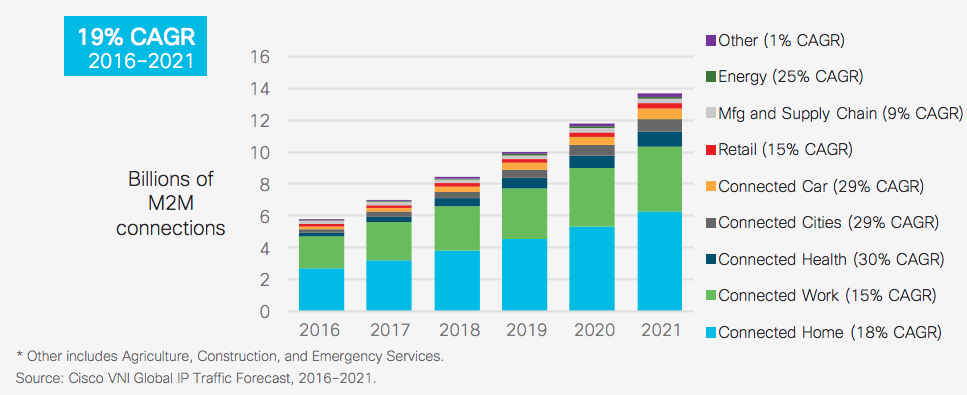
\includegraphics[width=1.0\textwidth]{m2mGrowth}
	\caption*{Fonte: \cite{ciscoReport}}
\label{fig:m2mGrowth}
\end{figure}

As oportunidades trazidas pelo conceito de \wiot{} à área de automação residencial são uma grande motivação para esse projeto. Também destaca-se a possibilidade de promover tais conhecimentos ao mercado nacional, com a criação de produtos e a sua adequação às necessidades dos potenciais consumidores brasileiros. Mesmo nos Estados Unidos, ainda é necessário tempo até que as casas conectadas se consolidem, de modo que há uma conjuntura propícia ao pioneirismo, com a criação de tecnologias de \wiot{} à preços acessíveis, capazes de serem absorvidos pela demanda de mercados emergentes.

\section{Projeto Hedwig}

\subsection{Objetivo}
A contribuição do projeto para o avanço das tecnologias de Internet das Coisas fundamenta-se na criação de um sistema com arquitetura modularizada, e em camadas, com funcionalidades locais e de nuvem, provendo uma API que permita seu acesso por diversos clientes --- como websites ou aplicativos para smartphones --- que seja capaz de monitorar e agir em diversos módulos presentes na residência do usuário final do sistema. O projeto irá disponibilizar módulos físicos, prontos para serem instalados e configurados na residência, sem que sejam necessários conhecimentos avançados de eletrônica ou computação.

Para a elaboração do projeto, e o alinhamento das expectativas e requisitos que o motivaram, os seguintes conceitos desempenharam papéis relevantes:

\begin{description}
\item \textbf{Robustez}

Com foco na robustez e disponibilidade, devem ser previstos níveis de operação para o sistema, os quais dispõem de diferentes requisitos de funcionalidades para garantir serviços essenciais, mesmo na ocorrência de problemas como a queda do servidor local, indisponibilidade de internet, falha no roteador, dentre diversas outras possibilidades. Há medidas tratativas, nos diferentes níveis, para a tentativa automática de reconexão, monitoramento de estado e manutenções preventivas e corretivas do sistema.

\item \textbf{Modularidade}

A modularidade, principalmente relacionada aos dispositivos físicos e as decisões arquiteturais, promove a independência de funcionamento entre as partes, e contribui no atendimento aos requisitos de robustez e disponibilidade. Em relação aos dispositivos, também representa diminuição nos custos de produção, e a possibilidade de que dispositivos específicos sejam desenvolvidos para aplicações diversas.

\item \textbf{Camadas}

A arquitetura do projeto é concebida em camadas e níveis, cujas responsabilidades são independentes. Cada parte do sistema exercita um conjunto de tarefas específicas (de transporte, análise, tomada de ações, etc.), e seus efeitos são traduzidos em entradas para o nível seguinte.

\item \textbf{Aprendizado de máquina}

Geração de aprendizado de máquina por meio de análise automática do uso do sistema pelos usuários, de forma a entender suas rotinas e poder atuar no conhecimento obtido, com notificações, alertas e acionamentos automáticos de funções para o usuário.

\item \textbf{Segurança}

A proteção da privacidade do usuário é tão importante, ou talvez mais, quanto a proteção física da casa. Assim, necessita-se que o sistema seja seguro, e que o fluxo de dados trocados entre as partes ocorra em meios protegidos. Foram utilizadas protocolos criptográficcos modernos para a proteção da troca de mensagens entre servidor local e serviços de nuvem. Todo usuário é autenticado e autorizado por meio de \emph{tokens} seguros, ao utilizar o aplicativo cliente, e a comunicação interna da casa é realizada em canais restritos.

\end{description}

\subsection{Nome do projeto}
O nome do projeto foi escolhido em homenagem a Hedy Lamarr. Nascida Hedwig Eva Maria Kiesler \cite{shearer}, a atriz e inventora desenvolveu, durante a Segunda Guerra Mundial, um aparelho de interferência em rádio para despistar radares nazistas, cujos princípios estão incorporados nas tecnologias atuais de Wi-Fi, CDMA e Bluetooth \cite{electronicFrontier}. Baseado na ideia de um sistema de comunicação seguro, e como reconhecimento de seu trabalho, foi dado esse nome ao projeto aqui descrito.

\subsection{Logo}
O logo do projeto é uma coruja, em referência à coruja Hedwig do personagem Harry Potter, da série de livros de mesmo nome. A coruja é responsável por encaminhar mensagens de maneira segura entre os interlocutores, assim como o projeto desenvolvido promove uma maneira segura de comunicação com sua casa.

\begin{figure}[H]
	\centering
	\caption{Logotipo do projeto Hedwig}
  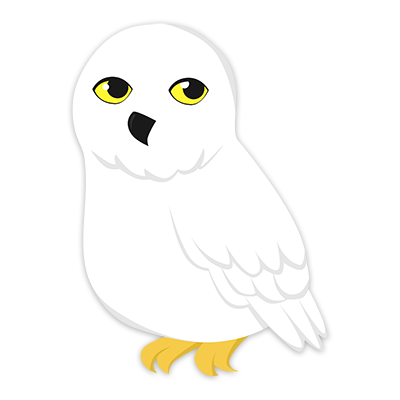
\includegraphics[width=0.35\textwidth]{hedwigLogo}
\label{fig:hedwigLogo}
\end{figure}

\section{Aplicações}
Como aplicações do projeto Hedwig, destacam-se a automação no uso de eletrodomésticos e iluminação, segurança no acesso à casa, economia nas contas de energia elétrica, além de  monitoramento remoto de pessoas que moram sozinhas, principalmente pessoas idosas, garantindo a tranquilidade de seus familiares e mantendo a segurança do indivíduo.

Exemplos de módulos que podem ser incluídos no sistema são: quarto (despertador, iluminação, monitoramento de temperatura e umidade); cozinha (\textit{timer}, iluminação, monitoramento de presença e gás); acesso (controle de abertura, monitoramento de estado); externo (monitoramento de temperatura, umidade, energia elétrica e consumo de água); corredor (monitoramento de presença, iluminação); chuveiro (controle de temperatura\slash potência a partir do perfil de usuário e temperatura externa) e ar condicionado (controle da potência a partir do monitoramento das temperaturas internas e externas da casa).

A presença de funcionalidades de aprendizado de máquina incrementa o sistema, traz facilidades e promove maior adaptação às rotinas dos moradores. O sistema é capaz de aprender com \emph{feedbacks} do usuário, seja pelo monitoramento dos módulos ou por respostas dadas pelo aplicativo, podendo atuar em questões de segurança (\emph{safety}), personalizações e até mesmo em possíveis sugestões de produtos relacionados aos hábitos do cliente.
